%%Uncomment for lecture version
\documentclass[aspectratio=169]{beamer}
\usepackage{pgfpages}
%\setbeameroption{show notes on second screen=right}
%%Uncomment for handouts
%\documentclass[aspectratio=169, handout]{beamer}
\usepackage{./diegobeamer,mylistings}
\usepackage{datetime2}
\usepackage{tikz}
\usepackage{booktabs}
\usepackage{wrapstuff}
\usepackage{numprint}
\usepackage{wrapfig}
\usepackage{amsfonts}
\usepackage{mathpartir}
%\usepackage{marginnote}
% \usepackage{enumitem}
\usetikzlibrary{positioning,decorations.pathreplacing,fit, calc}
%\documentclass[aspectratio=169, notes=only]{beamer}
%\documentclass[notes]{beamer}       % print frame + notes
% Common settings for all lectures in this course
\usepackage{hyperref}
\usepackage{makecell}
\usepackage{array}
\usepackage{tcolorbox}
\renewcommand\UrlFont{\color{blue}\rmfamily}
\usepackage{amssymb}
\usepackage{amsmath}
\usepackage{numprint}
\usepackage{paralist}
\usepackage{stmaryrd}
\usepackage{listings, xcolor}
\tikzset{hl/.style={
    set fill color=red!80!black!40,
    set border color=red!80!black,
  },
}
\usepackage{tcolorbox}

\tcbuselibrary{listings}
\tcbuselibrary{skins}

%\definecolor{verylightgray}{rgb}{.97,.97,.97}

\lstdefinelanguage{Solidity}{
	keywords=[1]{anonymous, assembly, assert, balance, break, call, callcode, case, catch, class, constant, continue, constructor, contract, debugger, default, delegatecall, delete, do, else, emit, event, experimental, export, external, false, finally, for, function, gas, if, implements, import, in, indexed, instanceof, interface, internal, is, length, library, log0, log1, log2, log3, log4, memory, calldata, modifier, new, payable, pragma, private, protected, public, pure, push, require, return, returns, revert, selfdestruct, send, solidity, storage, struct, suicide, super, switch, then, this, throw, transfer, true, try, typeof, using, value, view, while, with, addmod, ecrecover, keccak256, mulmod, ripemd160, sha256, sha3}, % generic keywords including crypto operations
	keywordstyle=[1]\color{blue}\bfseries,
	keywords=[2]{address, bool, byte, bytes, bytes1, bytes2, bytes3, bytes4, bytes5, bytes6, bytes7, bytes8, bytes9, bytes10, bytes11, bytes12, bytes13, bytes14, bytes15, bytes16, bytes17, bytes18, bytes19, bytes20, bytes21, bytes22, bytes23, bytes24, bytes25, bytes26, bytes27, bytes28, bytes29, bytes30, bytes31, bytes32, enum, int, int8, int16, int24, int32, int40, int48, int56, int64, int72, int80, int88, int96, int104, int112, int120, int128, int136, int144, int152, int160, int168, int176, int184, int192, int200, int208, int216, int224, int232, int240, int248, int256, mapping, string, uint, uint8, uint16, uint24, uint32, uint40, uint48, uint56, uint64, uint72, uint80, uint88, uint96, uint104, uint112, uint120, uint128, uint136, uint144, uint152, uint160, uint168, uint176, uint184, uint192, uint200, uint208, uint216, uint224, uint232, uint240, uint248, uint256, var, void, ether, finney, szabo, wei, days, hours, minutes, seconds, weeks, years},	% types; money and time units
	keywordstyle=[2]\color{teal}\bfseries,
	keywords=[3]{block, blockhash, coinbase, difficulty, gaslimit, number, timestamp, msg, data, gas, sender, sig, value, now, tx, gasprice, origin},	% environment variables
	keywordstyle=[3]\color{violet}\bfseries,
	identifierstyle=\color{black},
	sensitive=false,
	columns=flexible,
	comment=[l]{//},
	morecomment=[s]{/*}{*/},
	commentstyle=\color{gray}\ttfamily,
	stringstyle=\color{red}\ttfamily,
	morestring=[b]',
	morestring=[b]"
}

\lstdefinestyle{solidity_style}
{
	language=Solidity,
	%backgroundcolor=\color{verylightgray},
	extendedchars=true,
	basicstyle=\footnotesize\ttfamily,
	showstringspaces=false,
	showspaces=false,
	%numbers=left,
	numberstyle=\footnotesize,
	numbersep=9pt,
%    xleftmargin=5.0ex,	
    tabsize=2,
	breaklines=true,
	showtabs=false,
	captionpos=b,
	escapechar=!
}

\newtcblisting{soliditybox}[1][]{%
listing only,
listing options={language=Solidity, style=solidity_style, tabsize=2,escapeinside={(*@}{@*)}},
enhanced,
title=Solidity,
arc=1mm,
attach boxed title to top right = {xshift=-.5mm,yshift=-5.95mm},
boxed title style={size=small,arc=1mm, boxrule=0pt, sharp corners=downhill},
#1
}
\def\solidityinline{\lstinline[language=Solidity, style=solidity_style]}

\DeclareMathOperator{\dsum}{+}
\newcommand{\fromString}[1]{\ensuremath{\left\lceil#1\right\rceil}}
\newcommand{\toString}[1]{\ensuremath{\left\lfloor#1\right\rfloor}}
\newcommand{\update}[3]{
	\ensuremath{#1[#2\mapsto #3]}
}
\newcommand{\option}[1]{
	\ensuremath{#1}_\bot
}
\newcommand{\astack}[1]{\ensuremath{\mathit{sck}(#1)}}
\newcommand{\amemory}[1]{\ensuremath{\mathit{mem}(#1)}}
\newcommand{\astorage}[1]{\ensuremath{\mathit{sto}(#1)}}
\newcommand{\aaccount}[1]{\ensuremath{\mathit{acc}(#1)}}
\newcommand{\ustack}[2]{\ensuremath{\mathit{upSck}(#1,#2)}}
\newcommand{\umemory}[2]{\ensuremath{\mathit{upMem}(#1,#2)}}
\newcommand{\ustorage}[2]{\ensuremath{\mathit{upSto}(#1,#2)}}
\newcommand{\uaccount}[2]{\ensuremath{\mathit{upAcc}(#1,#2)}}
\newcommand{\Mod}[2]{#1~\mathrm{mod}~#2}

\newcommand{\tikzmark}[2][]{%
  \tikz[remember picture,overlay,baseline=-.5ex] \node[#1] (#2) {};%
}
% \drawBrace[xshift]{beginningNode}{endingNode}
% This command draws a brace between two tikzmarks, to their right,
% no matter which one is the rightmost, and includes 
% a node midway the brace, to write the comment.
% This command also creates a new node
% Whose name is the concat of the names of beginning and ending nodes.
\newcommand*{\drawBrace}[4][0pt]{%
    \node[draw=none, fit={(#2) (#3)}, inner sep=0pt] (rectg) {};%
    \draw [decoration={brace,amplitude=0.3em},decorate,very thick,red]%
      ([xshift=#1]rectg.north east) --%
      coordinate[right=.5em, midway] (#2#3)
      ([xshift=#1]rectg.south east);%
    \node[right=.4em of #2#3,align=left] (#2#3-comment) {#4};
    \draw (#2#3-comment.west) edge (#2#3);
}%
\def\lecturename{Computer Languages and Representations}
\def\lecturecode{ECM2418}
\def\coauthor{Achim D. Brucker}

\title{Secure Smart Contracts with Isabelle/Solidity}
%\subtitle{Secure Smart Contracts with Isabelle/Solidity}
\author{Diego Marmsoler, Asad Ahmed, Achim D. Brucker}

\institute
{
  Department of Computer Science\\
  University of Exeter
}

\lecture[1]{Introduction}{introduction}
\date{\DTMdisplaydate{2022}{03}{30}{-1}}
\makeatletter
\def\blfootnote{\gdef\@thefnmark{}\@footnotetext}
\makeatother
\begin{document}
\begin{frame}[plain,noframenumbering]
\maketitle
\bigskip
\bigskip
%\begin{center}
%
\includegraphics[width=1.5 in]{logo.PNG}
%\end{center}
\begin{tikzpicture}[remember picture, overlay]
\node[yshift=-3cm] at (current page.center) 
{
    
\includegraphics[width=1.5 in]{logo.PNG}
};
\end{tikzpicture}
\end{frame}

\frame{\tableofcontents}

\section{introduction}
\frame{\tableofcontents[currentsection]}

\subsection{Blockchain Technology}

\begin{frame}{Blockchain Technology}
\begin{itemize}
\item A database concept which relies upon decentralization and cryptography to store and retrieve the related database for transparency, immutability and security
\end{itemize}
 \tikz \node at (0, 3) [font=\large,   minimum height=2.5em, minimum width = 3.25cm, inner sep=0pt, fill=blue!30] {Application Layer};
\tikz \node [font=\normalsize, minimum height=2.5em, align = left] {Buisness logic for:\\[0.5pt]  Finance, Medical, Business, Agriculture etc};\\
\tikz \node [font=\large,  minimum height=2.5em, minimum width = 3.25cm, inner sep=0pt, fill=green!30 ] {Contract Layer};
\tikz \node [font=\normalsize, minimum height=2.5em, align = left] {Programs in high-level languages to\\[0.5pt]  implement the buisness logic};\\
\tikz \node [font=\large,  minimum height=2.5em, minimum width = 3.25cm, inner sep=0pt, fill=blue!30] {Consensus layer};
\tikz \node [font=\normalsize, minimum height=2.5em, align = left] {Set of rules agreed upon to add a new block,\\[0.5pt] such as  Proof of Work (PoW)};\\
\tikz \node [font=\large,  minimum height=2.5em, minimum width = 3.25cm, inner sep=0pt, fill=blue!30] {Network Layer};
\tikz \node [font=\normalsize, minimum height=2.5em, align = left] {Handels the communciationa between nodes};\\
\tikz \node [font=\large,  minimum height=2.5em, minimum width = 3.25cm, inner sep=0pt, fill=blue!30] {Data Layer};
\tikz \node [font=\normalsize, minimum height=2.5em, align = left] {Data transections, Blocks, Cryptography};\\
\begin{itemize}
\item High-level programs enlarges the threat surface
\end{itemize}
\end{frame}
%
\subsection{Contract Layer}
\begin{frame}{Smart Contracts}

 \begin{itemize}
\item Programs wirtten in high-level languages
\item Allows to automate the transections in a Blockchain
\item Key feature is: once deployed cannot be modified
\item Solidity is the most popular high-level language to write smart contracts
\end{itemize}
\end{frame}

\subsection{Solidity}
\begin{frame}{Solidity Smart Contract}
	\begin{center}
	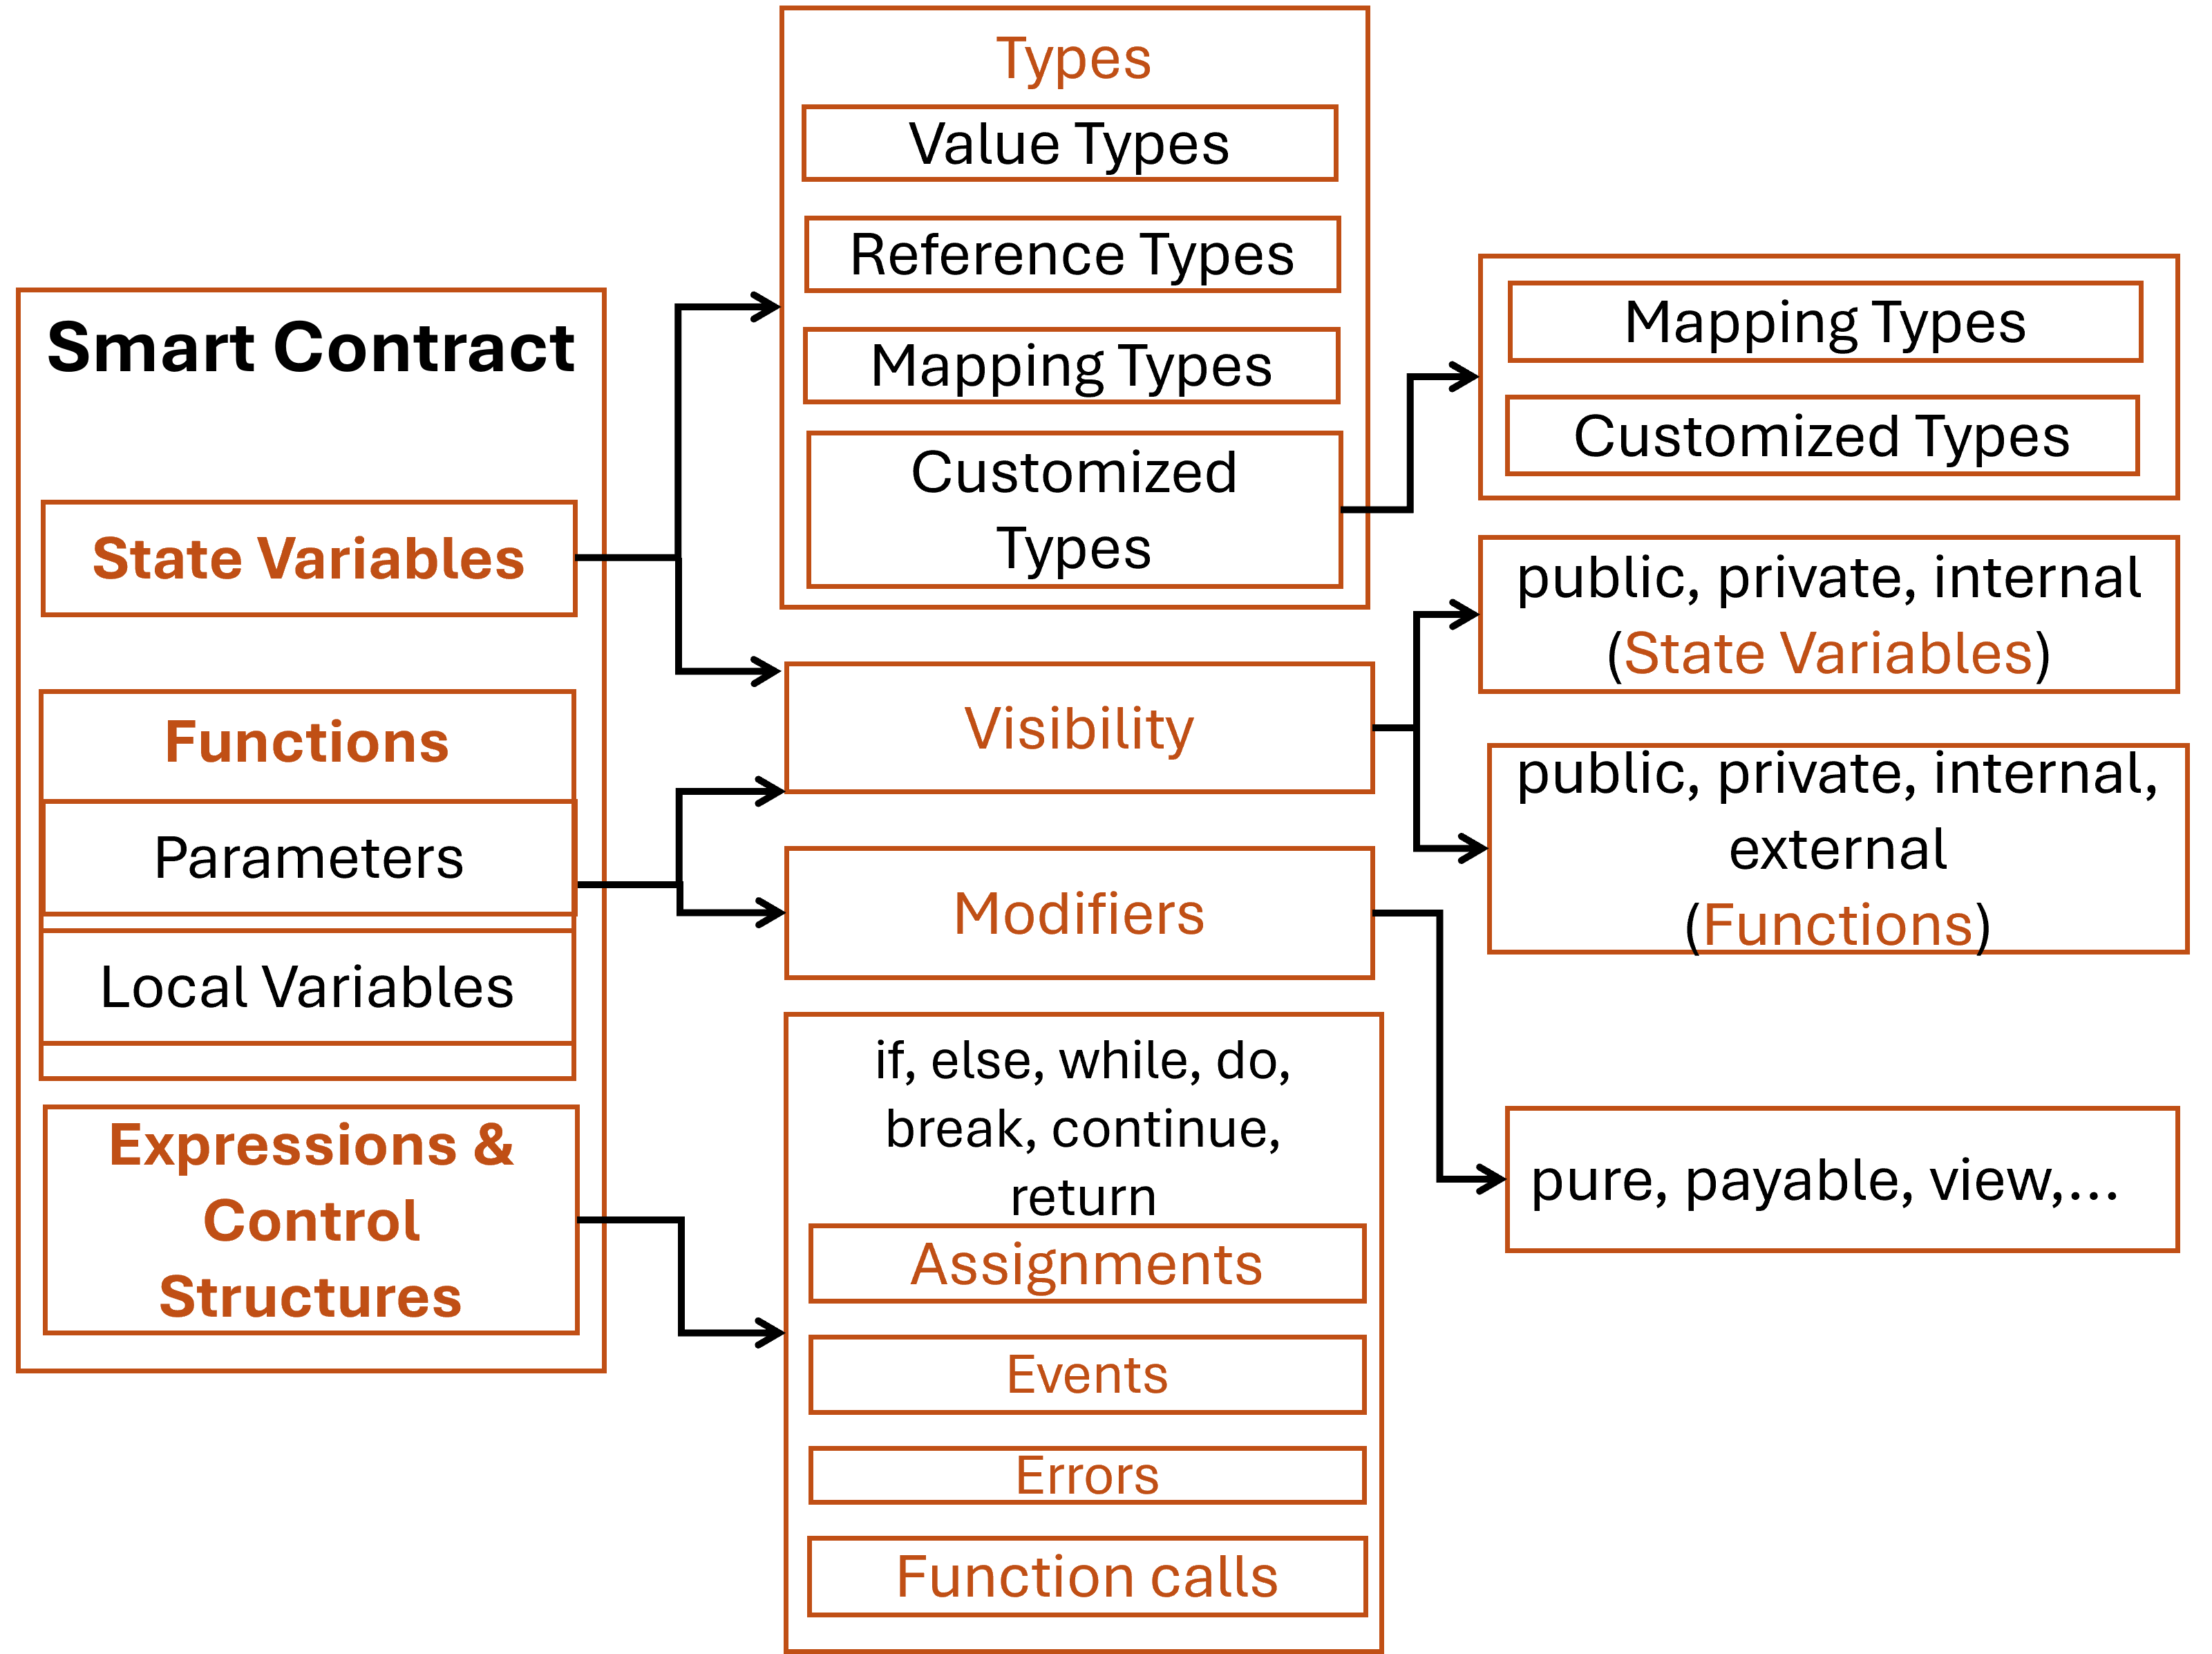
\includegraphics[width=10cm,keepaspectratio]{solidityl.PNG}
	\end{center}
\end{frame}
%
\begin{frame}{Solidity Store Types}
	\begin{center}
	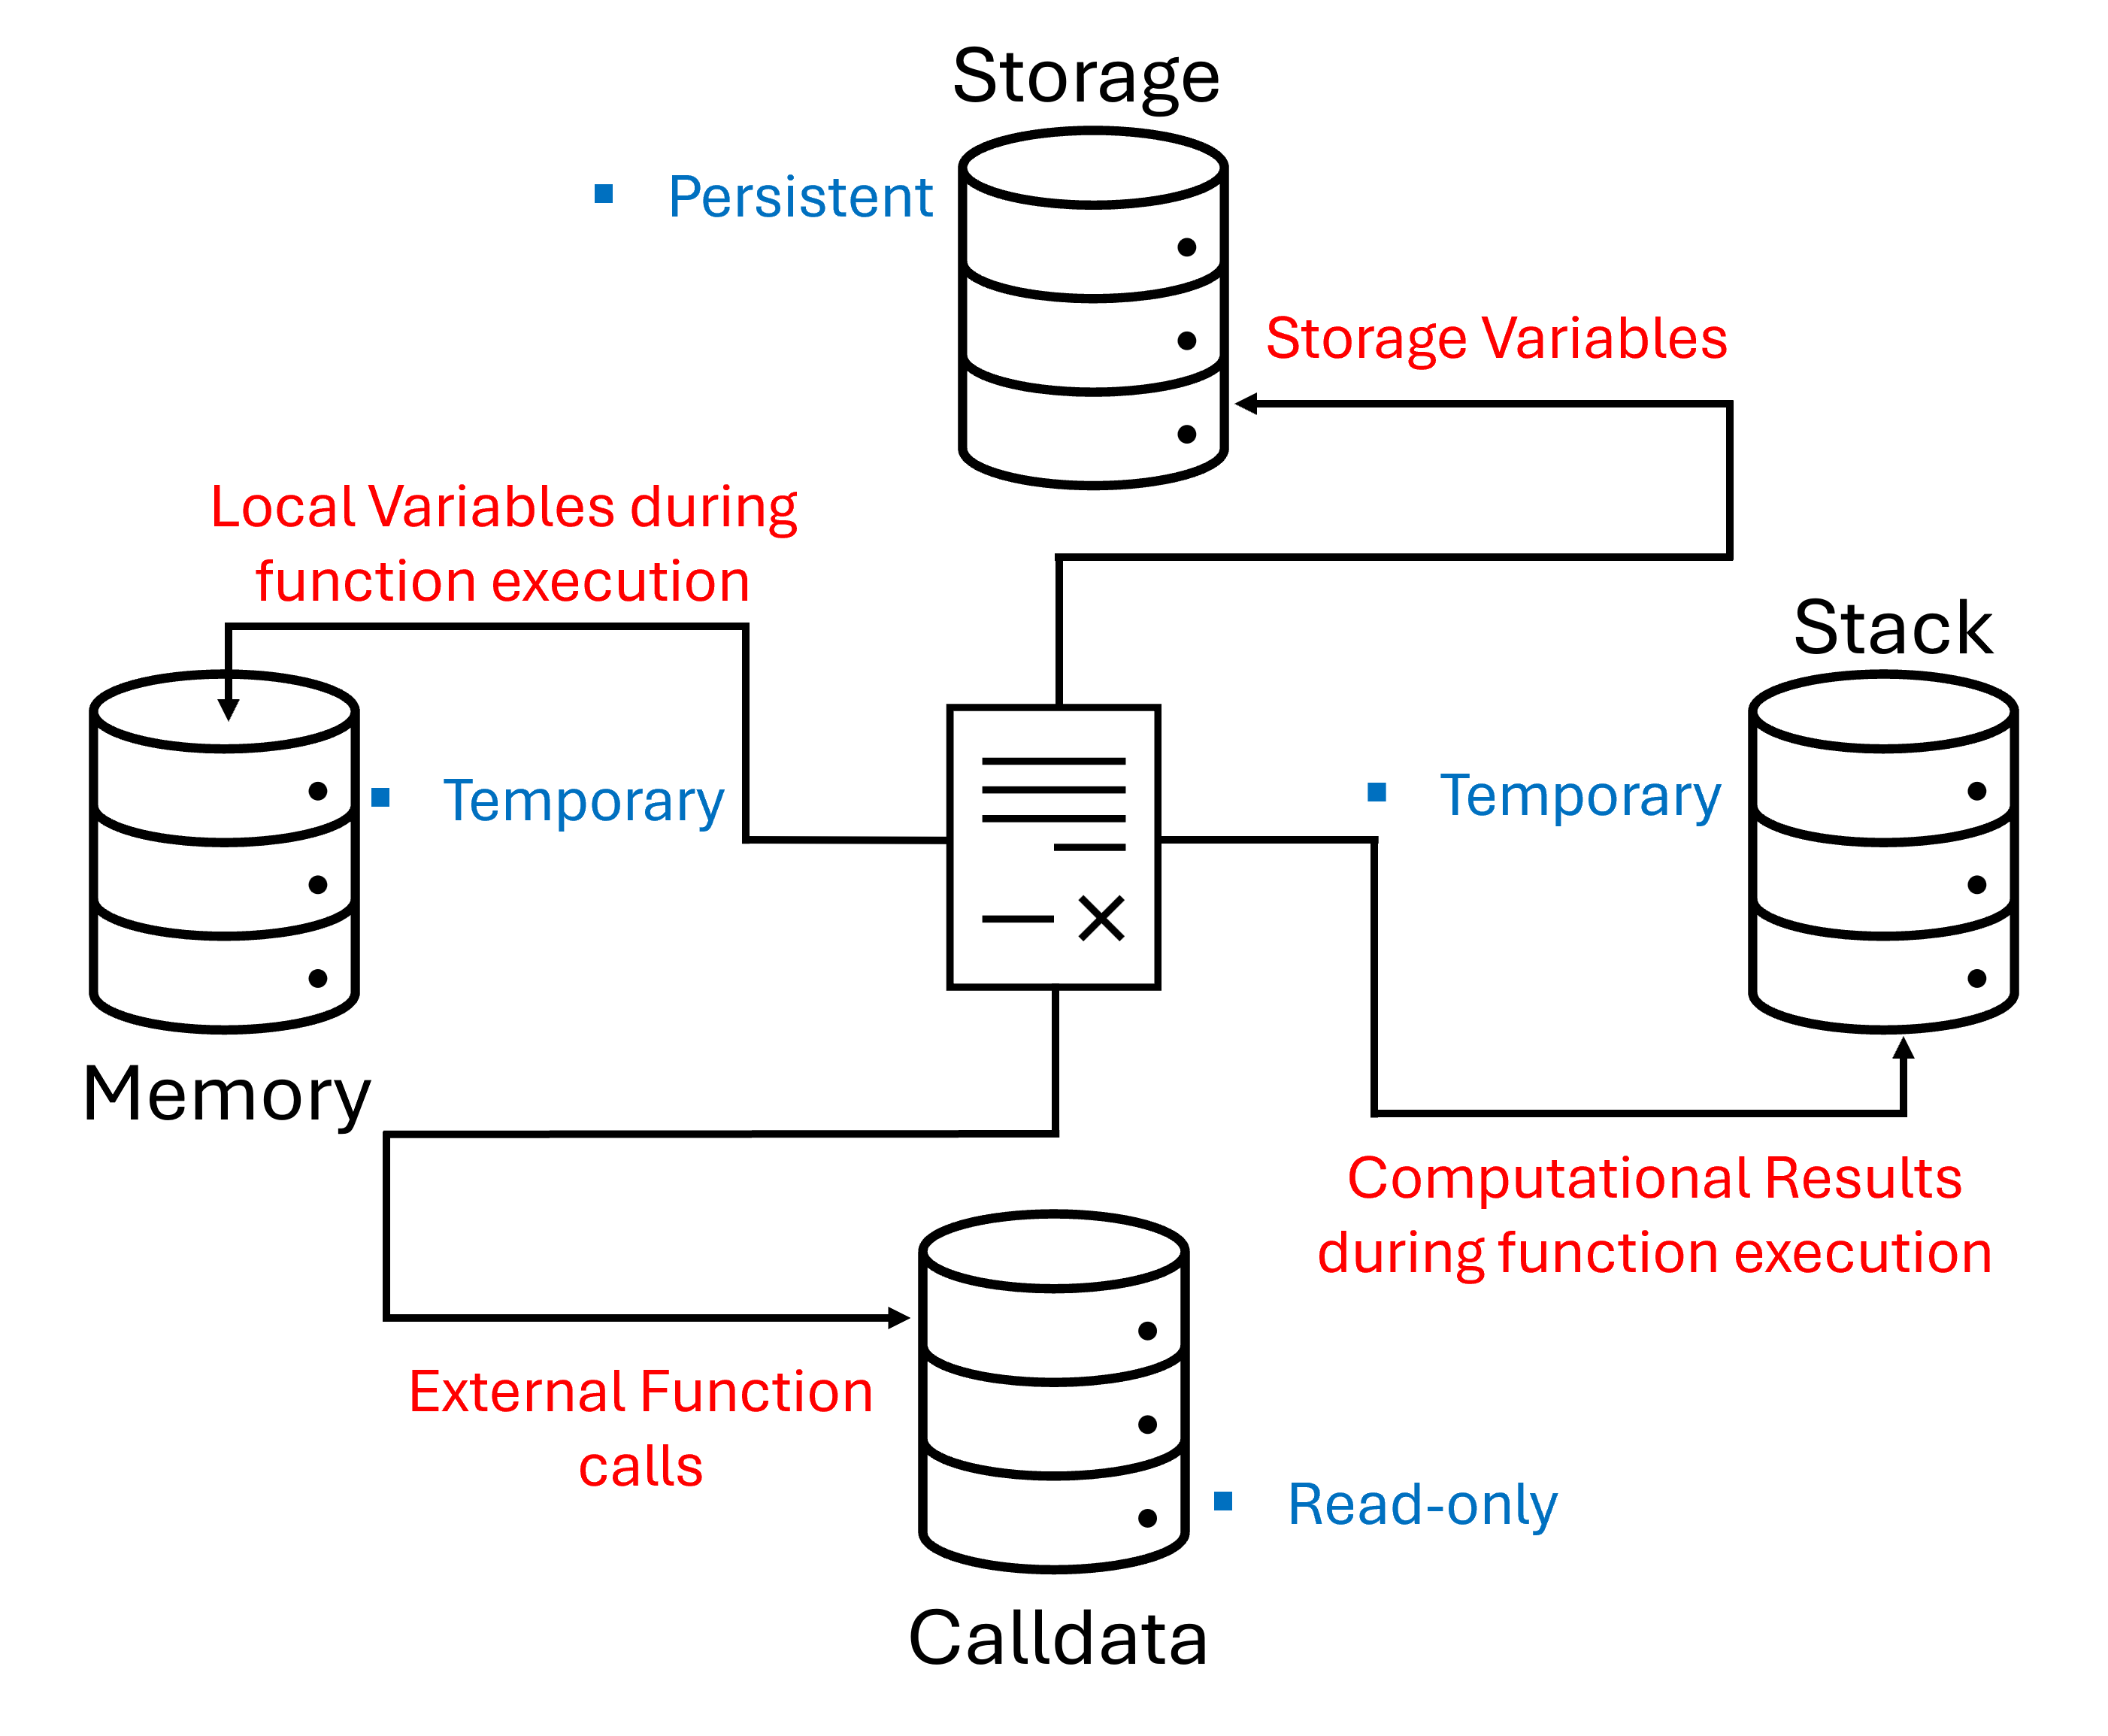
\includegraphics[width=7.5cm,keepaspectratio]{datatypes.PNG}
	\end{center}
\begin{exampleblock}{}
  {\large \begin{center}Storage types are a unique feature of Solidity \end{center}}
\end{exampleblock}
\end{frame}
%
\begin{frame}{Decentralized Autonomous Organization (DAO) smart contract}

 \begin{itemize}
\item Infamous malicious attack took place in 2016 
\item (DAO) smart contract was manipulated to steal around 2 Million Ether
\item Re-entrancy vulnerability
\end{itemize}
\vspace{0.5in}
\begin{exampleblock}{}
  {\large \begin{center}Errors and bugs in the smart contract programs lead to unbearable finanical losses \end{center}}
\end{exampleblock}
\end{frame}
\section{Related Work}
\begin{frame}{Related Work}
%
\begin{itemize}
%
\item{Axiomatic}
\begin{itemize}
\item[--] Solidity$^*$ \& EVM$^*$, SOLC-VERIFY, iCONTRACT e.t.c. 
\item[--] SMT Solvers, Modelchecking, KeY
\end{itemize}
%
%
\item{By-Construction}
\begin{itemize}
\item[--] SOLI, Denotational Sematic 
\item[--] Isabelle/HOL
\end{itemize}
%

\end{itemize}
\vspace{0.5in}
\begin{exampleblock}{}
  {\large \begin{center}To develop a theorem proving based light-weight formalization for specifying and verifying smart contracts\end{center}}
\end{exampleblock}
%\tikzmark{infrastructure}{A by-construction approach to develop a light-weight formalization framework for specifying and verifying smart contract}
%\vspace{-1.5in}
%\pause\tikz[overlay,remember picture]{\draw[draw=red, thick] ($(infrastructure)+(0,0.4)$) rectangle ($(infrastructure)+(9cm,0.4)$);}
\end{frame}

%\begin{frame}{Problem Statement}
%\end{frame}

\section{Proposed Methodology}
\begin{frame}{Proposed Methodology}
\begin{figure}[!h]
\centering
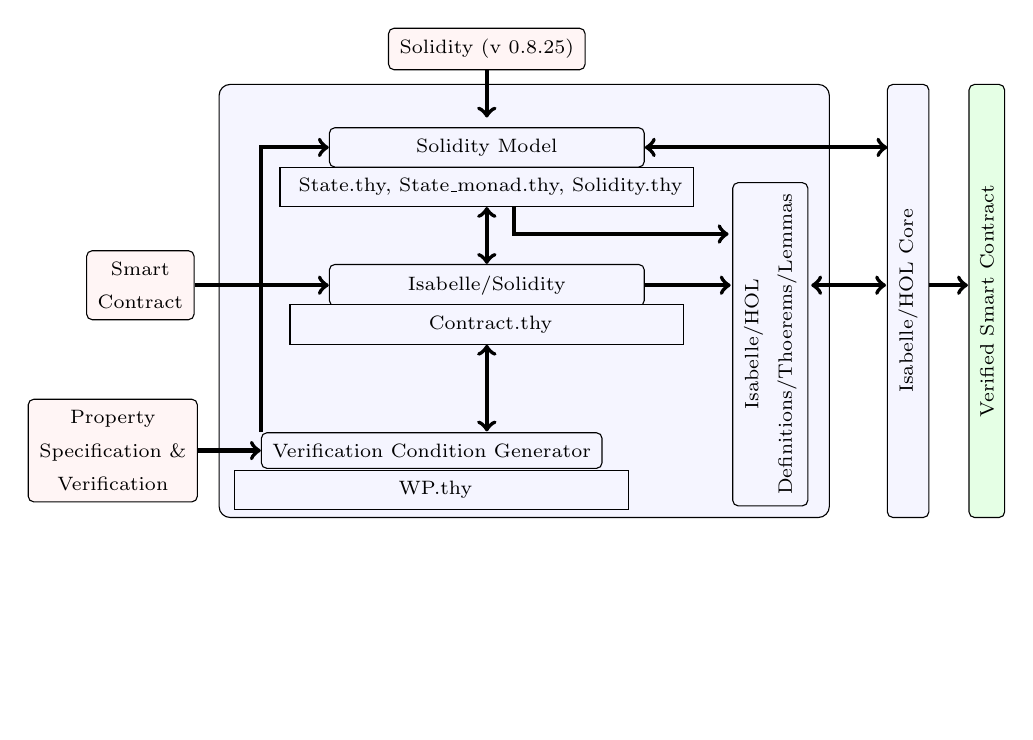
\begin{tikzpicture}
%PICTURE SCOPE or REFERENCEs
\node at (0, 0) (topleft) [circle] {};
%\node at (11.75, 0) (topright) [circle, draw=red, fill=red] {};
\node (topright) [circle, xshift = 10.5cm, right of = topleft] {};
\node (bottomleft) [circle, yshift = -7.25cm, below of = topleft] {};
\node (bottomright) [circle, xshift = 11.5cm, yshift = -7.25cm, below of = topleft] {};
%\draw (0,-3) [draw=red, fill=red]  -- (5, -4); % CHECK once of the grid is affecting the placement of the objects
%GRID

\draw (2, -0.45 ) [rounded corners = 4pt, draw=black, fill=blue!4]  -- ++(7.75cm, 0) --++(0, -5.5cm)--++(-7.75, 0)--cycle;
%\draw (2.5, -0.65) [rounded corners = 4pt, draw=black, fill=blue!4]  -- ++(5cm, 0) --++(0, -2.65cm)--++(-5, 0)--cycle;
%\draw (2.65, -0.85) [rounded corners = 4pt, draw=black, fill=blue!4]  -- ++(3.1cm, 0) --++(0, -2.3cm)--++(-3.1, 0)--cycle;
%INPUTS
\node (solidity) [thin, draw=black, fill=red!4,  rectangle, rounded corners= 2pt, xshift = 4.40cm, right of = topleft, inner sep = 4pt] {\scriptsize Solidity (v 0.8.25)};
\node (sc) [thin, draw=black, fill=red!4,  rectangle, rounded corners= 2pt, yshift = -3cm, right of = topleft, inner sep = 4pt, align = center] {\scriptsize Smart \\[0.15pt] \scriptsize Contract};
\node (scp) [thin, draw=black, fill=red!4,  rectangle, rounded corners= 2pt, xshift = -0.35cm, yshift = -5.10cm, right of = topleft, inner sep = 4pt, align = center] {\scriptsize Property  \\[0.15pt] \scriptsize  Specification \scriptsize \& \\[0.15pt]  \scriptsize  Verification};
%%THEORIES
\node (sm) [thin, draw=black, fill=blue!4,  rectangle, minimum width=4cm, rounded corners= 2pt, xshift = 4.40cm, yshift = -1.25cm, right of = topleft, inner sep = 4pt, align = center] {\scriptsize Solidity Model};
\node (sm1) [thin, draw=black, fill=blue!4,  rectangle, minimum width=4cm,  xshift = 4.40cm, yshift = -1.75cm, right of = topleft, inner sep = 4pt, align = center] {\scriptsize{ State.thy, State\_monad.thy, Solidity.thy}};
%
\node (isasol) [thin, draw=black, fill=blue!4,  rectangle, minimum width=4cm, rounded corners= 2pt, xshift = 4.40cm, yshift = -3cm, right of = topleft, inner sep = 4pt, align = center] {\scriptsize Isabelle/Solidity};
\node (isasol1) [thin, draw=black, fill=blue!4,  rectangle, minimum width=5cm,  xshift = 4.40cm, yshift = -3.50cm, right of = topleft, inner sep = 4pt, align = center] {\scriptsize{ Contract.thy}};
%
\node (vcg) [thin, draw=black, fill=blue!4,  rectangle, minimum width=4cm, rounded corners= 2pt, xshift = 3.70cm, yshift = -5.10cm, right of = topleft, inner sep = 4pt, align = center] {\scriptsize Verification Condition Generator};
\node (vcg1) [thin, draw=black, fill=blue!4,  rectangle, minimum width=5cm, xshift = 3.70cm, yshift = -5.60cm, right of = topleft, inner sep = 4pt, align = center] {\scriptsize{ WP.thy}};
%
\node (dtl) [thin, draw=black, fill=blue!4,  rectangle, minimum width=4cm, rounded corners= 2pt, xshift = 8cm, yshift = -3.75cm, right of = topleft, inner sep = 4pt, align = center, rotate=90] { {\scriptsize Isabelle/HOL}\\[0.15] {\scriptsize  Definitions/Thoerems/Lemmas}};
\node (isac) [thin, draw=black, fill=blue!4,  rectangle, rounded corners= 2pt, minimum width= 5.5cm, xshift = 9.75cm,  yshift= -3.2cm, right of = topleft,  inner sep = 4pt,   align = center, rotate=90] { {\scriptsize Isabelle/HOL Core}};
\node (vsc) [thin, draw=black, fill=green!10,  rectangle, rounded corners= 2pt, minimum width= 5.5cm, xshift = 10.75cm,  yshift= -3.2cm, right of = topleft,  inner sep = 4pt,   align = center, rotate=90] { {\scriptsize Verified Smart Contract}};
%%CONNECTIONS
\draw  [draw=black, line width = 1.5pt, ->] (sc.east) to [ out=360, in=180] (isasol.west);;
\draw  [draw=black, line width = 1.5pt, ->] (scp.east) to [ out=360, in=180] (vcg.west);;
%%INTERCONECTIONS
\draw  [draw=black, line width = 1.5pt, ->] (solidity.south) --  ++(0, -0.60cm) ;;
\draw  [draw=black, line width = 1.5pt, <->] (sm1.south)  to [out=270, in=90] (isasol.north);; ;;
\draw  [draw=black, line width = 1.5pt, <->] (isasol1.south)  to [out=270, in=90] ++(0, -1.10);; ;;
%%SM1 TO DTL
\draw  [draw=black, line width = 1.5pt, ->] (5.75, -2.35) -- ++(2.72cm, 0) ;;
\draw  [draw=black, line width = 1.5pt, -] (5.75, -2) -- ++(0, -0.38cm) ;;
\draw  [draw=black, line width = 1.5pt, ->] (isasol.east) -- ++(1.09cm, 0);;
%%SM TO HOL CORE
\draw  [draw=black, line width = 1.5pt, <->] (sm.east)  -- ++(3.08cm, 0);;;; ;;
%DTL TO CORE
\draw  [draw=black, line width = 1.5pt, <->] (9.52, -3) -- ++(0.95cm, 0) ;;
%%
\draw  [draw=black, line width = 1.5pt, ->] (11.01, -3) -- ++(0.5cm, 0) ;;
%%
\draw  [draw=black, line width = 1.5pt, ->] (vcg.north west) to [out=90, in=-90]   ++(0, 0.38cm)|- (sm.west) ;;
\end{tikzpicture}
\end{figure}
\end{frame}


\section{Isabelle/Solidity}
\frame{\tableofcontents[currentsection]}

%\begin{frame}{Bank}
%\begin{itemize}
%\item Keeps an internal record of funds transferred by its customers.
%\item This record is increased whenever a customer transfers additional funds 
%\item When customer withdraws all its recorded
%funds are returned and its internal record reset to 0.
%\end{itemize}
\subsection{Example Contract}
\begin{frame}{Banking}
\begin{tcolorbox}[colback=white,colframe=red!4,title=\textcolor{red}{Specification:}]
\begin{center} 
Simple smart contract in Solidity which allows clients to deposit and withdraw funds.
\end{center}
\end{tcolorbox} 
%\begin{soliditybox}
pragma solidity >=0.5.1 <0.5.2;

contract Bank {
    mapping(address => uint256) balances;

    function deposit() public payable {
        balances[msg.sender] = balances[msg.sender] + msg.value;
    }

    function withdraw() public {
        uint256 bal = balances[msg.sender];
        balance[msg.sender] = 0;
        msg.sender.transfer(bal);
    }
}
\end{soliditybox}
\begin{tcolorbox}[colback=white,colframe=red!4,title=\textcolor{red}{Property:}]
	\begin{align*}
		\mathit{Invariance}\colon&\mathit{\color{blue}balance} \geq \sum_{\{(a,x)|\texttt{balances}(a)=x\}} x\\
	\end{align*}
\end{tcolorbox} 
\end{frame}
%
\subsection{Solidity Specification}
\begin{frame}{Banking Smart Contract}

\begin{figure}[!h]
\centering
\begin{tikzpicture}
%PICTURE SCOPE or REFERENCEs
\node at (0, 0) (topleft) [circle] {};
%\node at (11.75, 0) (topright) [circle, draw=red, fill=red] {};
\node (topright) [circle, xshift = 10.5cm, right of = topleft] {};
\node (bottomleft) [circle, yshift = -7.25cm, below of = topleft] {};
\node (bottomright) [circle, xshift = 11.5cm, yshift = -7.25cm, below of = topleft] {};
%\draw (0,-3) [draw=red, fill=red]  -- (5, -4); % CHECK once of the grid is affecting the placement of the objects
%GRID
\node[] at (current page.center) 
{
  \begin{minipage}[t]{0.66\textwidth}
\begin{soliditybox}
pragma solidity >=0.5.1 <0.5.2;

contract Bank {
    mapping(address => uint256) balances;

    function deposit() public payable {
        balances[msg.sender] = balances[msg.sender] + msg.value;
    }

    function withdraw() public {
        uint256 bal = balances[msg.sender];
        balance[msg.sender] = 0;
        msg.sender.transfer(bal);
    }
}
\end{soliditybox}
\end{minipage}
};
\node (ssc) [xshift=-1.15cm, yshift=3.05cm, rectangle, draw=red, red, minimum width = 5.25cm, minimum height=0.75cm, thick] at (current page.center) 
{};
\node (ci) [xshift=-2.23cm, yshift=2.35cm, rectangle, draw=red, red, minimum width = 3cm, minimum height=0.35cm, thick] at (current page.center) 
{};
\node (map) [xshift=-0.10cm, yshift=1.9cm, rectangle, draw=red, red, minimum width = 6.25cm, minimum height=0.35cm, thick] at (current page.center) 
{};
\node (df) [xshift=-0.10cm, yshift=1.20cm, rectangle, draw=red, red, minimum width = 6.25cm, minimum height=0.35cm, thick] at (current page.center) 
{};
\node (dflogic) [xshift=0.250cm, yshift=0.58cm, rectangle, draw=red, red, minimum width = 6cm, minimum height=0.75cm, thick] at (current page.center) 
{};
\node (wflogic) [xshift=0.50cm, yshift=-1.90cm, rectangle, draw=red, red, minimum width = 6.25cm, minimum height=2cm, thick] at (current page.center) 
{};
%%LABELING
\node (sscl) [xshift=-6.15cm, yshift=3.05cm] at (current page.center) 
{Compiler Directive};
\node (cil) [xshift=-6.15cm, yshift=2.35cm] at (current page.center) 
{keyword $<$name$>$};
\node (mapl) [xshift=-6.15cm, yshift=1.9cm] at (current page.center) 
{type $<$name$>$};
\node (dfl) [xshift=-6.6cm, yshift=1.20cm] at (current page.center) 
{\scriptsize{keyword} $<$\scriptsize{name}$>$ \scriptsize{visibility} \scriptsize{modifier}};
\node (dflogicl) [xshift=-6.15cm, yshift=0.58cm] at (current page.center) 
{Deposit logic};
\node (wflogicl) [xshift=-6.15cm, yshift=-1.90cm] at (current page.center) 
{Withdraw logic};
%%CONNECTIONS
\draw  [draw=red, line width = 1.5pt, ->] (ssc.west) -- (sscl.east) ;;
\draw  [draw=red, line width = 1.5pt, ->] (ci.west) -- (cil.east) ;;
\draw  [draw=red, line width = 1.5pt, ->] (map.west) -- (mapl.east) ;;
\draw  [draw=red, line width = 1.5pt, ->] (df.west) -- (dfl.east) ;;
\draw  [draw=red, line width = 1.5pt, ->] (dflogic.west) -- (dflogicl.east) ;;
\draw  [draw=red, line width = 1.5pt, ->] (wflogic.west) -- (wflogicl.east) ;;
\end{tikzpicture}
\end{figure}
\end{frame}
%%
%%
\begin{frame}{Isabelle/Solidity Specification}

\begin{Example}{}{}
	The formalization of our example :
	\begin{center}
		\fbox{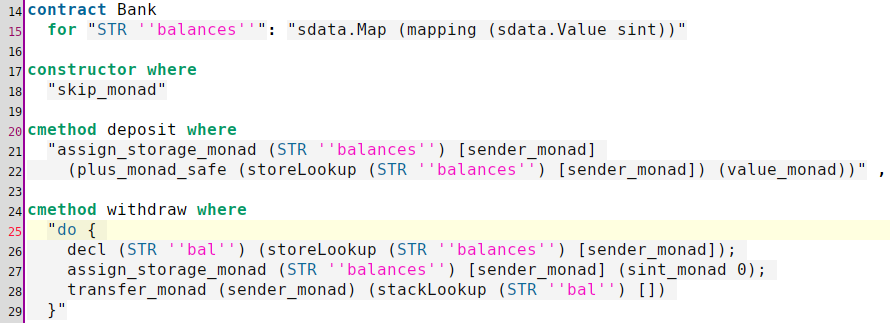
\includegraphics[width = 11.5cm]{bank_spec.png}}
	\end{center}
\end{Example}
\end{frame}
%%
%%
\begin{frame}{Isabelle/Solidity Statements Semantic}
\begin{columns}
\column{.48\textwidth}

\begin{itemize}
\item 
\item
\end{itemize}

\column{.48\textwidth}
\begin{table}[]

\caption{Assignments for complex data types}\label{tab:assign}

\begin{tabular}{ccc}
 M& M & S \\
M &  C&  D   \\
 M&  P&  D \\
M &  S&  D\\
S & M&   D\\
S & C&   D\\
S & P&   D\\
S & S& D\\
P& S& S\\
P&M&N/A\\
P&C&N/A\\
P&P&N/A\\
C&--&N/A
\end{tabular}
\end{table}
\end{columns}
\end{frame}

%%
%%
\begin{frame}{Isabelle/Solidity Verification}
\begin{Example}{}{}
\begin{align*}
		\mathit{Invariance}\colon&\mathit{\color{blue}balance} \geq \sum_{\{(a,x)|\texttt{balances}(a)=x\}} x\\
	\end{align*}
		\begin{center}\vspace{-2mm}
		\fbox{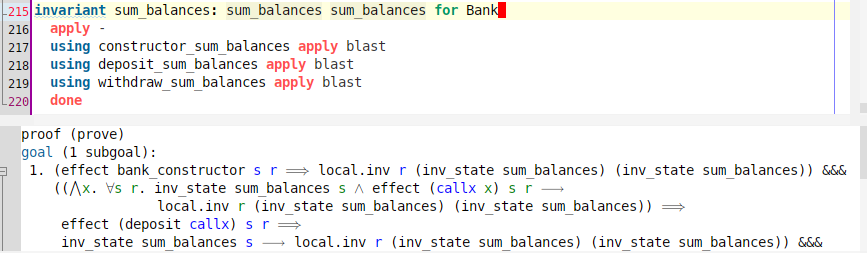
\includegraphics[width=.95\textwidth]{invariant.png}}
	\end{center}\vspace{-2mm}
Output window shows proof obligations discharged using lemmas.
\end{Example}
\end{frame}
%
\subsection{Isabelle/Solidity Specification \& Verification}

\begin{frame}{Isabelle/Solidity Specification }
	\begin{figure}[!h]
\centering
\begin{tikzpicture}
%PICTURE SCOPE or REFERENCEs

\node[] at (current page.center) 
{
  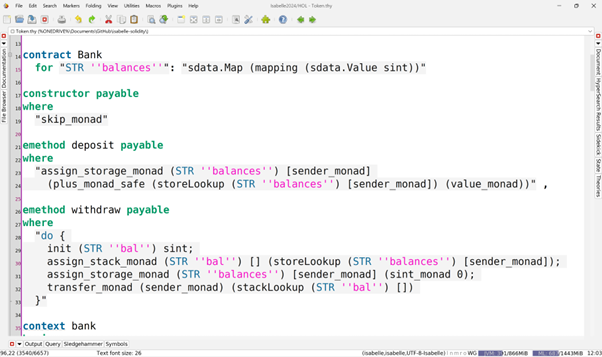
\includegraphics[width=\textwidth]{isasol.PNG}
};
\node (issol-ci) [xshift=-1.65cm, yshift=2.5cm, rectangle, draw=green, red, minimum width = 8.75cm, minimum height=0.90cm, thick] at (current page.center) 
{};
\node (issol-con) [xshift=-4.80cm, yshift=1.45cm, rectangle, draw=green, red, minimum width = 2.55cm, minimum height=1cm, thick] at (current page.center) 
{};
\node (issol-f) [xshift=0cm, yshift=0.30cm, rectangle, draw=green, red, minimum width = 12cm, minimum height=1.15cm, thick] at (current page.center) 
{};
%%LABELS
\node (issol-cil) [xshift=1.75cm, yshift=4cm] at (current page.center) 
{\small{keyword $<$name$>$ store keyword  $<$variable name$>$: $<$ type$>$}};
\node (issol-conl) [xshift=1.75cm, yshift=1.5cm] at (current page.center) 
{\small{keyword  modifier keyword $<$body$>$}};
\node (issol-fl) [xshift=1.75cm, yshift=-1.25cm] at (current page.center) 
{\small{keyword $<$name$>$ modifier keyword $<$body$>$}};
%%CONNECTIONS
\draw  [draw=red, line width = 1.5pt, ->] (issol-ci.north east) -- (issol-cil.south) ;;
\draw  [draw=red, line width = 1.5pt, ->] (issol-con.east) -- (issol-conl.west) ;;
\draw  [draw=red, line width = 1.5pt, ->] (issol-f.south) -- (issol-fl.north) ;;
\end{tikzpicture}
\end{figure}
\end{frame}
%%
\begin{frame}{Isabelle/Solidity Specification }
	\begin{figure}[!h]
\centering
\begin{tikzpicture}
%PICTURE SCOPE or REFERENCEs

\node[] at (current page.center) 
{
  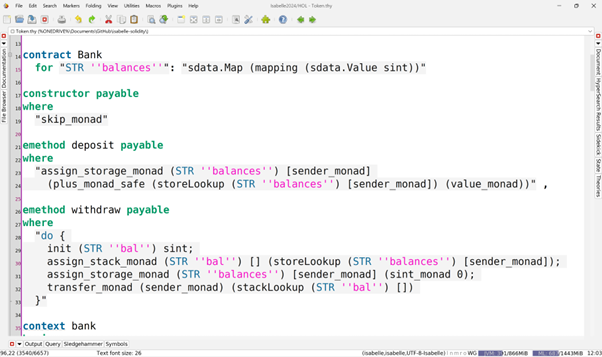
\includegraphics[width=\textwidth]{isasol.PNG}
};
%\node (issol-ci) [xshift=-1.65cm, yshift=2.5cm, rectangle, draw=green, red, minimum width = 8.75cm, minimum height=0.90cm, thick] at (current page.center) 
%{};
\node (sdata) [xshift=-4.40cm, yshift=2.35cm, rectangle, draw=green, red, minimum width = 2.85cm, minimum height=0.5cm, thick] at (current page.center) 
{};
\node (assignstore) [xshift=-4.30cm, yshift=0.300cm, rectangle, draw=green, red, minimum width = 2.75cm, minimum height=0.5cm, thick] at (current page.center) 
{};
\node (slu) [xshift=-2.30cm, yshift=-0.25cm, rectangle, draw=green, red, minimum width = 1.75cm, minimum height=0.5cm, thick] at (current page.center) 
{};
\node (stack) [xshift=-4cm, yshift=-1.50cm, rectangle, draw=green, red, minimum width = 3.1cm, minimum height=0.30cm, thick] at (current page.center) 
{};
\node (assignstack) [xshift=-4cm, yshift=-1.75cm, rectangle, draw=green, red, minimum width = 3.1cm, minimum height=0.30cm, thick] at (current page.center) 
{};
\node (stacklu) [xshift=-0.50cm, yshift=-2.350cm, rectangle, draw=green, red, minimum width = 2cm, minimum height=0.30cm, thick] at (current page.center) 
{};
%%LABELS
%\node (issol-cil) [xshift=1.75cm, yshift=4cm] at (current page.center) 
%{\small{keyword $<$name$>$ store keyword  $<$variable name$>$: $<$ type$>$}};
\node (sdatal) [xshift=1.75cm, yshift=1.5cm] at (current page.center) 
{\small{storage variable}};
\node (stackl) [xshift=0cm, yshift=-1.250cm] at (current page.center) 
{\small{stack variable}};
%%CONNECTIONS
%\draw  [draw=red, line width = 1.5pt, ->] (issol-ci.north east) -- (issol-cil.south) ;;
\draw  [draw=red, line width = 1.5pt, ->] (sdata.east) -- (sdatal.west) ;;
\draw  [draw=red, line width = 1.5pt, ->] (sdatal.west) -- (assignstore.north) ;;
%\draw  [draw=red, line width = 1.5pt, ->] (assignstore.south) -- (slu.west) ;;
\draw  [draw=red, line width = 1.5pt, ->] (assignstore.south) -- (slu.west) ;;
\draw  [draw=red, line width = 1.5pt, ->] (stack.east) -- (stackl.west) ;;
\end{tikzpicture}
\end{figure}
\end{frame}
%%


\begin{frame}{Isabelle/Solidity Verification }
	\begin{figure}[!h]
\centering
\begin{tikzpicture}
%PICTURE SCOPE or REFERENCEs

\node[] at (current page.center) 
{
  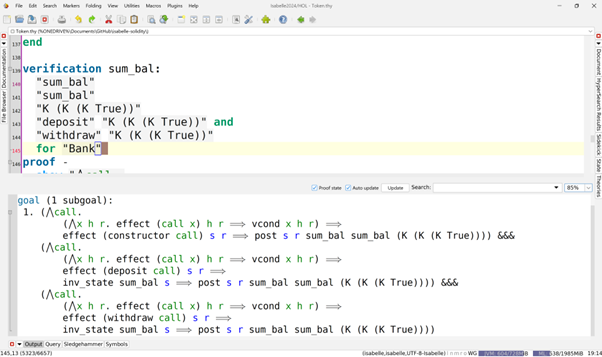
\includegraphics[width=0.95\textwidth]{ver.PNG}
};
\node (ver) [xshift=-3.46cm, yshift=1.5cm, rectangle, draw=green, red, minimum width = 4.5cm, minimum height=2.15cm, thick] at (current page.center) 
{};
\node (po) [xshift=-0.5cm, yshift=-2.15cm, rectangle, draw=green, red, minimum width = 12cm, minimum height=3.15cm, thick] at (current page.center) 
{};
%%LABEL
\node (verl) [xshift=3cm, yshift=1.5cm] at (current page.center) 
{  \begin{minipage}[t]{0.25\textwidth}
	\begin{align*}
	\mathit{\color{blue}balance} \geq \sum_{\{(a,x)|\texttt{balances}(a)=x\}} x\\
	\end{align*}
\end{minipage}};
\node (pol) [xshift=-0.20cm, yshift=-0.25cm] at (current page.center) 
{Proof Obligations};
\end{tikzpicture}
\end{figure}

\end{frame}
%%%
\section{Example Applications}
\frame{\tableofcontents[currentsection]}

\subsection{Verified Constant Solving}
\begin{frame}{Verified Constant Solving}
\begin{columns}
\column{.48\textwidth}
\begin{soliditybox}
int16 x;

// costs 20 Gas
x = int16(250) + uint8(500);

// costs 8 Gas
x = int16(494);
\end{soliditybox}

\bigskip\pause

\begin{center}
We implemented a constant solver for Solidity in Isabelle/HOL and verified that it preserves the semantic of a program.
\end{center}

\column{.48\textwidth}
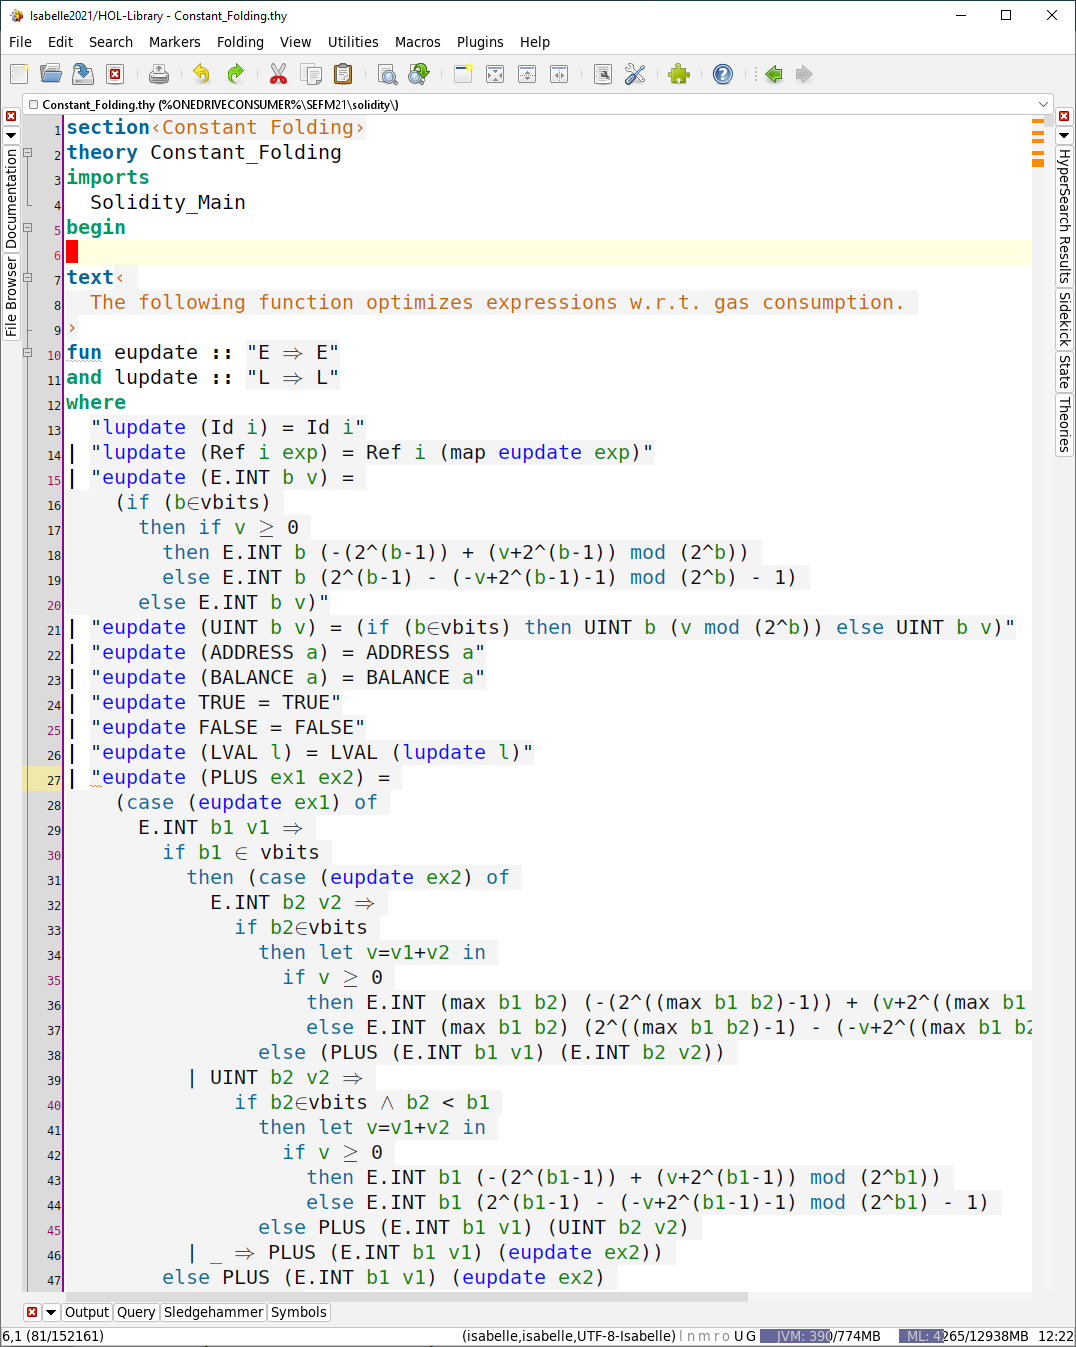
\includegraphics[width=\columnwidth]{isacs}
\end{columns}
\end{frame}

\subsection{Verification of Simple Token}
\begin{frame}{Functional Verification of (very) Simple Token}
\begin{lstlisting}[style=solidity_style, escapechar=!, basicstyle=\tiny, mathescape]

contract Bank{	!\tikzmark{bgnIBVar}!
    	  mapping(uint16 => uint8) balances; !\tikzmark{trmIBVar}!
        function deposit() public payable { !\tikzmark{bgnIBUVar}!
        balances[msg.sender] = balances[msg.sender] + msg.value;!\tikzmark{trmIBUVar}!
             }
   function withdraw() public payable { 
	...!\tikzmark{bgnTR}!      
	uint256 bal = balances[msg.sender];
	balances[msg.sender] = 0;
	msg.sender.transfer(bal);
	...!\tikzmark{trmTR}!
                  }
         }
}!\mbox{%
\begin{tikzpicture}[overlay, remember picture]
    \drawBrace[1cm]{bgnIBVar}{trmIBVar}{Initializing \\balance variable};
    \drawBrace[1cm]{bgnIBUVar}{trmIBUVar}{Transfering money\\ in account};
    \drawBrace[4cm]{bgnTR}{trmTR}{Transfering money \\out of account};
%    \drawBrace[8cm]{bgnWF}{trmWF}{Withdraw function};
%   \drawBrace[8cm]{bgnDF}{trmDF}{Deposit function};
% %   \drawBrace[1cm]{bgnState}{trmState}{Generated\\ input state};
  %  \drawBrace[7cm]{bgnCode}{trmCode}{Generated\\ program};
   % \drawBrace[4cm]{bgnAss}{trmAss}{Computed \\ result state};
  \end{tikzpicture}}!
\end{lstlisting}
  

\end{frame}

\begin{frame}{Functional Verification of (very) Simple Token}
	For both methods we verified the following pre- / postconditions:
	\begin{align*}
		\mathit{pre(\alert{b})}\colon&\mathit{\color{blue}balance}-\sum_{\{(a,x)|\texttt{balances}(a)=x\}} x \geq \mathit{\alert{b}}\\
		\mathit{post(\alert{b})}\colon&\mathit{\color{blue}balance}-\sum_{\{(a,x)|\texttt{balances}(a)=x\}} x \geq \mathit{\alert{b}}
	\end{align*}
\pause

	Note that withdraw triggers the execution of fallback methods which is code we do \emph{not} know yet
	\begin{itemize}
		\item In particular we verified that the above holds \emph{for every possible implementation} of fallback methods
		\item This is possible with Isabelle using structural induction over the implementation of the fallback method
	\end{itemize}
\end{frame}

\section{Conclusion}
\frame{\tableofcontents[currentsection]}

\begin{frame}{Conclusion}
Summary
\begin{itemize}
	\item Deep embedding of subset of Solidity in Isabelle/HOL
	\item Executable semantics with automatic conformance testing
	\item Used to create verified tools for Solidity
	\item Used to verify concrete Solidity contracts
\end{itemize}
\bigskip\pause

Limitations: Semantics
\begin{itemize}
	\item Some advanced features are still missing: inheritance
	\item Based on v0.5.16
\end{itemize}
\bigskip\pause

Limitations: Verification
\begin{itemize}
	\item Reasoning from semantic definitions is tedious
	\item Low degree of automation
	\item Example: Simple token required more than $3000$ lines of proof code
\end{itemize}
\end{frame}

\begin{frame}{Project Proposal}
	Aim: A verified tool which takes as input an annotated Solidity contract and generates a verification condition which can be discharged in Isabelle/HOL
	\bigskip\pause

	Objectives
	\begin{itemize}
		\item Develop a calculus to reason about semantics and implement it in Isabelle
		\item Implement a Verification Condition Generator
		\item Organize a smart contract verification competition
	\end{itemize}
	\bigskip\pause

	Team
	\begin{itemize}
		\item Myself: Work on semantics
		\item Prof. Achim Brucker: Expert in Isabelle
		\item Postdoc (to be funded by the grant)
		\item PhD student (funded by University of Exeter)
	\end{itemize}
\end{frame}

\begin{frame}{Possibilities for Collaboration}
	Required: A supporting statemement for the proposal
	\begin{itemize}
		\item Confirmation that the project is interesting
		\item Usually some (unbinding) commitment for some type of support\\
		(usually in terms of time spent on the project)
	\end{itemize}
	\bigskip\pause

	Desired: Ongoing discussions, feedback, ideas
	\begin{itemize}
		\item Regular meetings to discuss progress
		\item Insights into practical examples
		\item Feedback about usability
		\item Ideas for improvements
		\item Collaboration on publications
	\end{itemize}
\end{frame}

\begin{frame}[allowframebreaks]{References}
	\nocite{*}
	\bibliographystyle{unsrt}
	\bibliography{references.bib}
\end{frame}

\end{document}